\documentclass[mathserif]{beamer}

\setbeamertemplate{frametitle}[default][center]%Centers the frame title.
\setbeamertemplate{navigation symbols}{}%Removes navigation symbols.
\setbeamertemplate{footline}{\raisebox{5pt}{\makebox[\paperwidth]{\hfill\makebox[10pt]{\scriptsize\insertframenumber}}}}

\usepackage{amsmath,amssymb,amsthm}
\usepackage{graphicx,array,dsfont}
\usepackage{harvard}
\citationmode{abbr}

\newcommand{\Hrule}{\rule{\linewidth}{0.2pt}}
\newcommand{\argmax}{\mathop{\mathrm{argmax}}}
\newcommand{\argmin}{\mathop{\mathrm{argmin}}}
\newcommand{\minimize}{\mathop{\mathrm{minimize}}}
\def\half{\frac{1}{2}}
\def\th{\mathrm{th}}
\def\sign{\mathrm{sign}}
\def\supp{\mathrm{supp}}
\def\E{\mathrm{E}}
\def\P{\mathrm{P}}
\def\Var{\mathrm{Var}}
\def\Cov{\mathrm{Cov}}
\def\R{\mathds{R}} 
\def\cA{\mathcal{A}}
\def\cB{\mathcal{B}}
\def\cE{\mathcal{E}}
\def\cF{\mathcal{F}}
\def\cG{\mathcal{G}}
\def\cN{\mathcal{N}}
\def\red{\color[rgb]{0.8,0,0}}
\def\white{\color[rgb]{1,1,1}}

\begin{document}

%% Lecture was too short 
%% But with R examples, it was fine

\title{Information retrieval}
\author{Rebecca C. Steorts \\ Predictive Modeling: STA 521}
\date{September 1 2015}

\begin{frame}
\titlepage
\end{frame}

\begin{frame}
\frametitle{What we use to do}
I want to learn about that magic trick with the rings!

\bigskip
{\red Then: go to the library}
\begin{center}
\begin{tabular}{ccc}
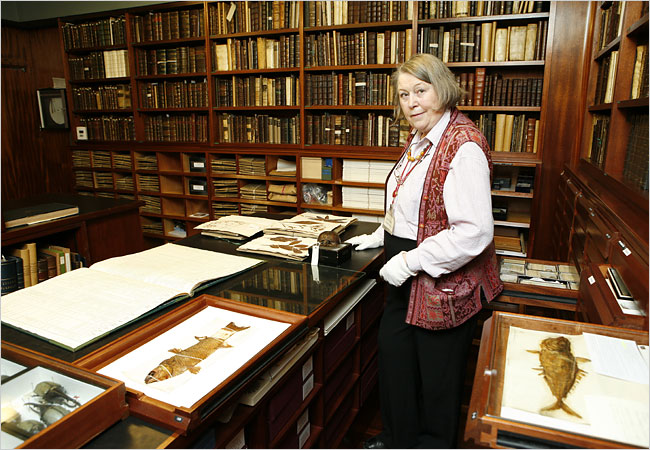
\includegraphics[height=1in]{librarian.jpg} & 
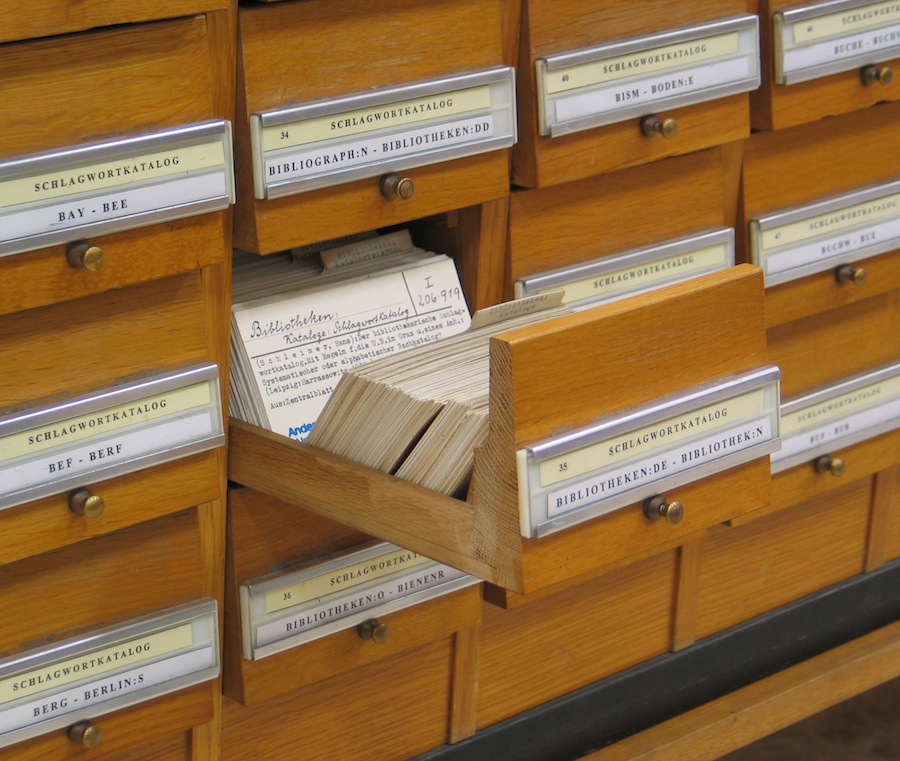
\includegraphics[height=1in]{catalog.jpg} & 
\hspace{-12pt}
\setlength\fboxsep{0pt}
\setlength\fboxrule{0.5pt}
\fbox{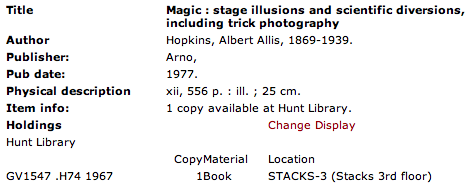
\includegraphics[height=0.5in]{metadata.png}} \\
Librarian & Card catalog & Metadata
\end{tabular}
\end{center}

\bigskip
Slow and expensive ...
\end{frame}

\begin{frame}
\frametitle{What we do now}
{\red Now: search the web!}
\begin{center}
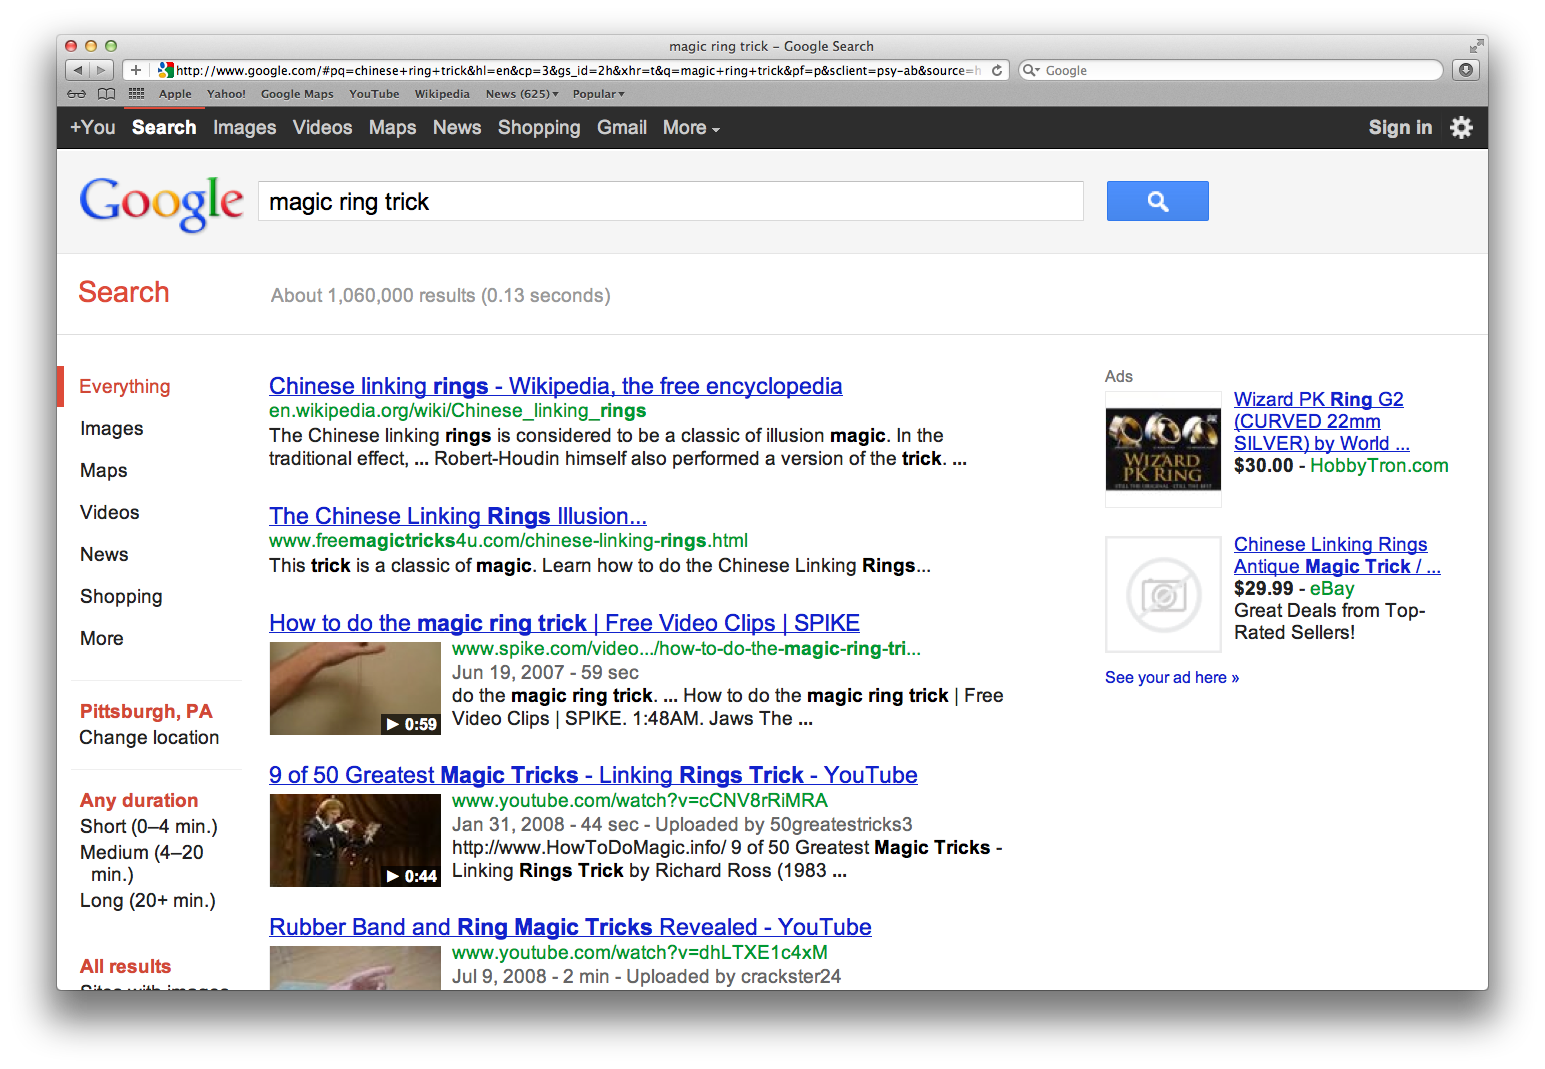
\includegraphics[height=0.7\textheight]{googlesearch.png}
\end{center}

\vspace{-10pt}
How did Google do this?
\end{frame}

\begin{frame}
\frametitle{Information retrieval and representations}
{\red Information retrieval}:
given a set of documents (e.g., webpages), 
our problem is to pull up the $k$ most similar documents 
to a given query (e.g., ``magic ring trick'')

\bigskip
First step is to think of a way of {\red representing}
these documents. We want our representation to:
\begin{itemize}
\item Be easy to generate from the raw documents, and 
be easy to work with
\item Highlight important aspects of the documents, and
suppress unimportant aspects
\end{itemize}

\bigskip
There is kind of a {\red trade-off} between these two ideas
\end{frame}

\begin{frame}
\frametitle{Try using the meaning of documents}
\begin{tabular}{cc}
\hspace{-15pt}
\parbox{0.5\textwidth}{
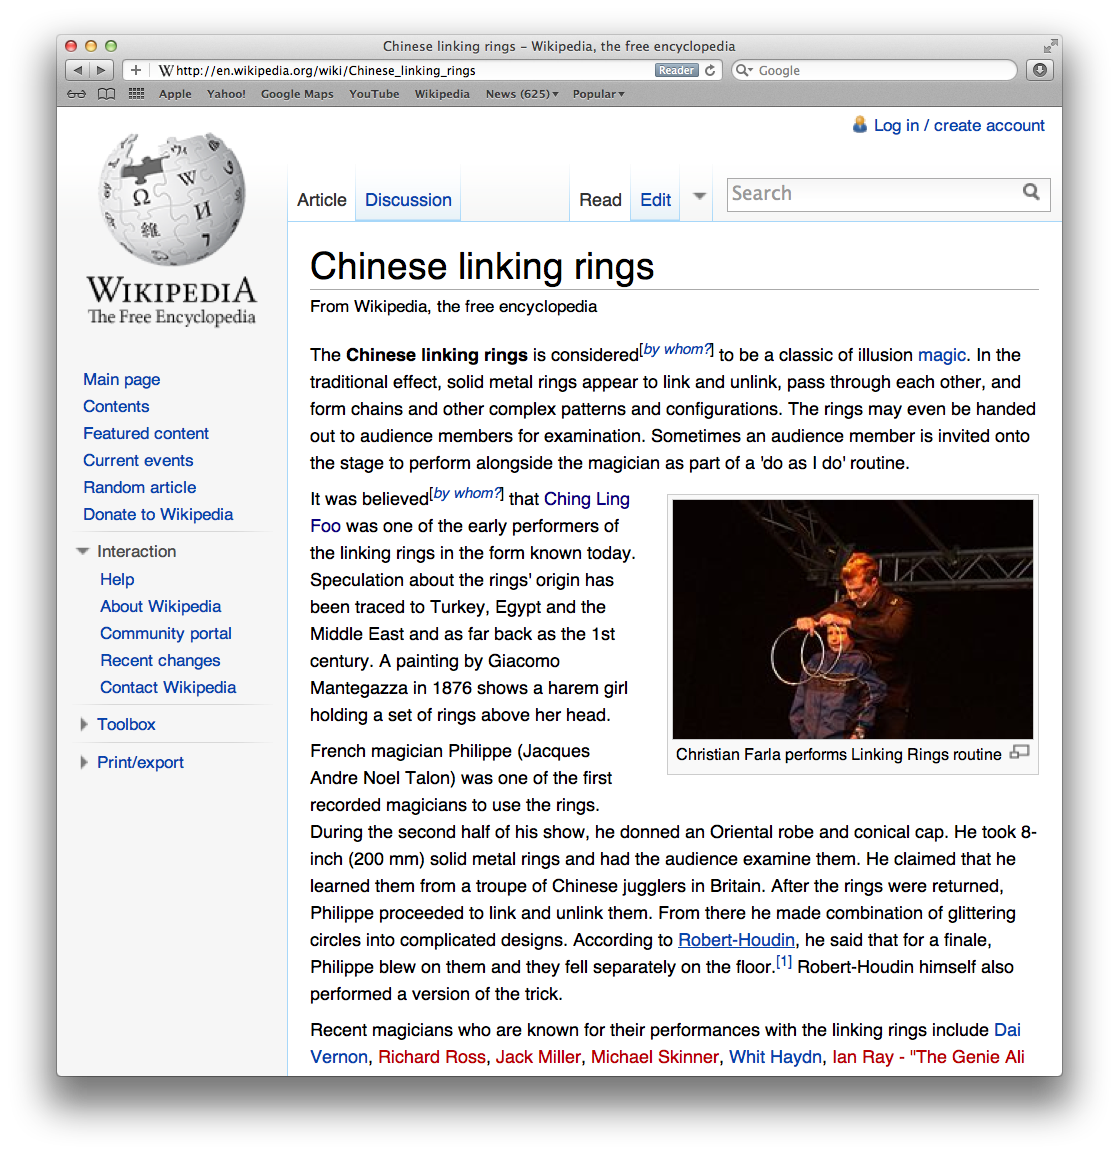
\includegraphics[width=0.5\textwidth]{wikipedia.png}} & 
\parbox{0.5\textwidth}{
What if we tried to represent the {\red meaning} of 
documents? E.g., 

\bigskip
{\footnotesize\tt 
type.of.trick = sleight of hand; \\
date.of.origin = 1st century; \\
place.of.origin = Turkey, Egypt; \\
name.origin = Chinese jugglers in Britain; ...}

\bigskip
This would be good in terms of our second idea 
(useful and efficient data reduction), but not our first
one ({\red extremely hard} to generate, 
and even hard to use!)}
\end{tabular}
\end{frame}

\begin{frame}
\frametitle{Bag-of-words representation}
{\red Bag-of-words} representation of 
a document is very simple-minded: just list all the words and 
how many times they appeared. E.g.,

\vspace{-5pt}
\begin{center}
{\footnotesize\tt
magic = 29; ring = 34; trick = 6; illusion = 7; link = 9; ...}
\end{center}

\vspace{-5pt}
Very easy to generate and easy to use (first idea),
but is it too much of a reduction, or can it still be useful 
(second idea)?

\bigskip
Idea: by itself ``ring'' can take on a 
lot of meanings, but we can learn from the {\red other words}
in the document besides ``ring''. E.g.,
\begin{itemize}
\item Words ``perform'', ``illusion'', ``gimmick'', 
``Chinese'', ``unlink'', ``audience'', ``stage'' 
suggest the right type of rings
\item Words ``diamond'', ``carat'', ``gold'', 
``band'', ``wedding'', ``engagement'', ``anniversary''
suggest the wrong type 
\end{itemize}
\end{frame}

\begin{frame}
\frametitle{Counting words}
Recall problem: given a query and a set of documents, 
find the $k$ documents most similar to the query

\bigskip
Counting words:
\begin{itemize}
\item First make a list of all of the words present in the 
documents and the query
\item
Index the words $w = 1,\ldots W$ (e.g., in alphabetical 
order), and the documents $d=1,\ldots D$ (just pick some 
order)
\item For each document $d$, count how many times
each word $w$ appears (could be zero), and call this $X_{dw}$. 
The vector $X_d = (X_{d1},\ldots X_{dW})$ gives 
us the {\red word counts} for the $d$th document
\item Do the same thing for the query: let $Y_w$ be the number of  
times the $w$th word appears, so the vector $Y=(Y_1,\ldots Y_W)$
contains the word counts for the query
\end{itemize}
\end{frame}

\begin{frame}
\frametitle{Simple example}
{\red Documents}: 
\begin{center}
1: ``Beka loves statistics.'' and 
2: ``Noah hates, hates statistics!''
\end{center}
{\red Query}: ``hates statistics''

\bigskip
$D=2$ documents and $W=5$ words total.
For each document and query, we count the number of 
occurences of each word:

\begin{center}
\begin{tabular}{|c|c|c|c|c|c|}
\hline
 & hates & Beka & loves & Noah & statistics \\
\hline
$X_1$ & 0 & 1 & 1 & 0 & 1 \\
\hline
$X_2$ & 2 & 0 & 0 & 1 & 1 \\
\hline
$Y$ & 1 & 0 & 0 & 0 & 1 \\
\hline
\end{tabular}
\end{center}

\smallskip
This is called the {\red document-term} matrix
\end{frame}

\begin{frame}
\frametitle{Distances and similarity measures}
\smallskip
We represented each document $X_d$ and query $Y$ in 
a convenient vector format. Now how to measure 
{\red similarity} between vectors, or equivalently,
dissimilarity or {\red distance}?

\bigskip
Measures of distance between
$n$-dimensional vectors $X,Y$:
\begin{itemize}
\item The {\red $\ell_2$} or {\red Euclidean} distance
is 
\vspace{-5pt}
$$\|X-Y\|_2 = \sqrt{\sum_{i=1}^n (X_i-Y_i)^2}$$
\item The {\red $\ell_1$} or {\red Manhattan} distance
is 
\vspace{-5pt}
$$\|X-Y\|_1 = \sum_{i=1}^n |X_i-Y_i|$$
\end{itemize}

{\red Basic idea}: find $k$ vectors $X_d$ with the 
smallest $\|X_d - Y\|_2$

(Note: $\ell_1$ distance doesn't work as well here)
\end{frame}

\begin{frame}[fragile]
\frametitle{Bigger example}

\smallskip
\smallskip
{\red Documents}: 8 Wikipedia articles, 4 about 
the TMNT Leonardo, Raphael, Michelangelo, and Donatello, and
4 about the painters of the same name

\begin{center}
\vspace{-20pt}
\begin{tabular}{ccccccccc} 
\hspace{-10pt}

\includegraphics[width=0.4in]{leo.jpg} & 

\includegraphics[width=0.4in]{rap.jpg} &

\includegraphics[width=0.4in]{mic.jpg} &

\includegraphics[width=0.4in]{don.jpg} &
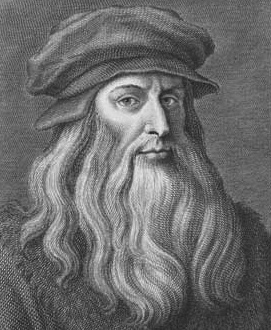
\includegraphics[width=0.4in]{leo2.jpg} &
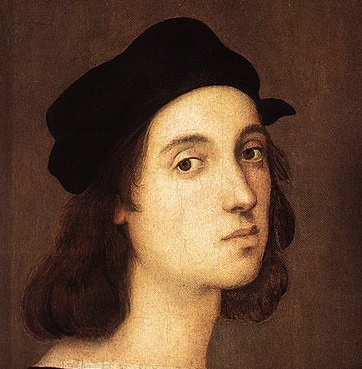
\includegraphics[width=0.4in]{rap2.jpg} &
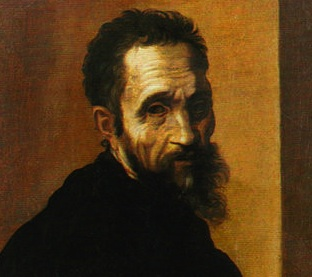
\includegraphics[width=0.4in]{mic2.jpg} &
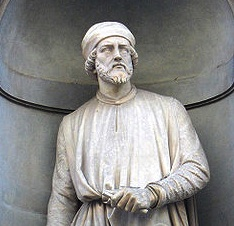
\includegraphics[width=0.4in]{don2.jpg} \\ 
1 & 2 & 3 & 4 & 5 & 6 & 7 & 8
\end{tabular}
\end{center}

\vspace{-5pt}
{\red Query}: ``Raphael is cool but rude, Michelangelo is a party dude!''

{\footnotesize
\begin{verbatim}
      but cool dude party michelangelo raphael rude ...    dist
doc 1  19    0    0     0            4      24    0     309.453
doc 2   8    1    0     0            7      45    1     185.183
doc 3   7    0    4     3           77      23    0     330.970
doc 4   2    0    0     0            4      11    0     220.200
doc 5  17    0    0     0            9       6    0     928.467
doc 6  36    0    0     0           17     101    0     646.474
doc 7  10    0    0     0          159       2    0     527.256
doc 8   2    0    0     0            0       0    0     196.140
query   1    1    1     1            1       1    1       0.000
\end{verbatim}}
\end{frame}

\begin{frame}[fragile]
\frametitle{Varying document lengths and normalization}
\smallskip
Different documents have different lengths. Total word counts:

\vspace{-5pt}
{\footnotesize
\begin{verbatim}
doc 1 doc 2 doc 3 doc 4 doc 5 doc 6 doc 7 doc 8 query 
 3114  1976  3330  2143  8962  6524  4618  1766     7 
\end{verbatim}}

\vspace{-5pt}
Wikipedia entry on Michelangelo the painter is almost twice as long
as that on Michelangelo the TMNT (6524 vs 3330 words). 
And query is only 7 words long! We should
{\red normalize} the count vectors $X_d$ and $Y$ in some way

\begin{itemize}
\item {\red Document length} normalization: divide $X$
by its sum,
\vspace{-5pt}
$$X \leftarrow X/\sum_{w=1}^W X_w$$
\item {\red $\ell_2$ length} normalization: divide $X$ 
by its $\ell_2$ length,
\vspace{-5pt}
$$X \leftarrow X / \|X\|_2$$
\end{itemize}

% apparently, normalizing by $\ell_2$ length tends 
% to better de-emphasize words that are rare in 
% the document.
\end{frame}

\begin{frame}[fragile]
\frametitle{Back to our Wikipedia example}
{\footnotesize
\begin{verbatim}
                 dist/doclen dist/l2len
doc 1 (tmnt leo)       0.385      1.373
doc 2 (tmnt rap)       0.378      1.322
doc 3 (tmnt mic)       0.378      1.319
doc 4 (tmnt don)       0.389      1.393
doc 5 (real leo)       0.390      1.405
doc 6 (real rap)       0.382      1.349
doc 7 (real mic)       0.381      1.325
doc 8 (real don)       0.393      1.411
query                  0.000      0.000
\end{verbatim}}

{\red Great!}

\bigskip
So far we've dealt with varying document lenghts.
What about some words being more helpful than
others? {\red Common words}, especially, are not
going to help us find relevant documents
\end{frame}

\begin{frame}
\frametitle{Common words and IDF weighting}
To deal with common words, we could just keep a list
of words like ``the'', ``this'', ``that'', etc. to
exclude from our representation. But
this would be both {\red too crude} and {\red time
consuming}

\bigskip
{\red Inverse document frequency (IDF)} weighting
is smarter and more efficient
\begin{itemize}
\item
For each word $w$, let $n_w$ be the number of 
documents that contain this word
\item
Then for each vector $X_d$ and $Y$, multiply 
$w$th component by 
$\log(D/n_w)$
\end{itemize}

\bigskip
If a word appears in every document, then it gets
a weight of zero, so effectively tossed out of the representation 

\bigskip
(Future reference: IDF performs something like
{\red variable selection})

% advantages: can get rid of unimportant variables
% disadvantages: could throw out too many features,
% with small collection of docs. Also, can downweight 
% or throw out informative features, e.g., all of our 
% articles could likely contain Michelangelo, but how 
% many times it appears is important!
\end{frame}

\begin{frame}
\frametitle{Putting it all together}
Think of the document-term matrix:

\smallskip
\begin{center}
\begin{tabular}{|c|c|c|c|c|}
\hline
& word 1 & word 2 & $\ldots$ & word $W$ \\
\hline
doc 1 & & & & \\
\hline
doc 2 & & & & \\
\hline
$\vdots$ & & & & \\
\hline
doc $D$ & & & & \\
\hline
\end{tabular}
\end{center}

\smallskip
\begin{itemize}
\item {\red Normalization} scales each row by something
(divides a row vector $X$ by its sum $\sum_{i=1}^W X_i$ 
or its $\ell_2$ norm $\|X\|_2$)
\item {\red IDF weighting} scales each column by something
(multiplies the $w$th column by $\log(D/n_w)$)
\item We can use both, just normalize first and then 
perform IDF weighting
\end{itemize}
\end{frame}

\begin{frame}[fragile]
\frametitle{Back to our Wikipedia example, again}
{\footnotesize
\begin{verbatim}
                 dist/doclen/idf dist/l2len/idf
doc 1 (tmnt leo)           0.623          1.704
doc 2 (tmnt rap)           0.622          1.708
doc 3 (tmnt mic)           0.620          1.679
doc 4 (tmnt don)           0.623          1.713
doc 5 (real leo)           0.622          1.693
doc 6 (real rap)           0.622          1.703
doc 7 (real mic)           0.622          1.690
doc 8 (real don)           0.624          1.747
query                      0.000          0.000
\end{verbatim}}

{\red Oops!} This didn't work as well as we might 
have hoped. Why? 

\bigskip
(Hint: our collection only contains
8 documents and 1 query ...)
\end{frame}

\begin{frame}
\frametitle{Stemming}
Having words ``connect'', ``connects'', ``connected''
``connecting'', ``connection'', etc. in our representation
is extraneous. {\red Stemming} reduces
all of these to the single stem word ``connect''

\bigskip
Can a simple list of rules provide perfect stemming? {\red
It seems not}: consider ``connect'' and ``connectivity'',
but ``relate'' and ``relativity''; or ``sand'' and ``sander'',
but ``wand'' and ``wander''.

\bigskip
Stemming also {\red depends on the language}. Apparently 
it is easier in English than it is in:
\begin{itemize}
\item German, a ``fusional'' language, e.g., 
\begin{center}
{\it Hubschrauberlandeplatz} = helicopter landing pad
\end{center}
\item Turkish, an ``agglutinative'' language, e.g.,
\begin{center}
{\it Turklestiremedigimizlerdensinizdir} = 
maybe you are one of those whom we were not able to 
Turkify'
\end{center}
\end{itemize}

% Advantages: reduce model complexity (dim reduction)
% disadvantages: could get rid of important features,
% e.g., ``Saturns'' probably indicates an article about 
% the car, not the planet
\end{frame}

\begin{frame}
\frametitle{Feedback}
People are usually better at {\red confirming the 
relevance} of something that's been found, rather 
than explaining what they're looking for in the 
first place

\bigskip
{\red Rocchio's algorithm} takes 
feedback from the user about relevance, and then
refines the query and repeats the search
\begin{enumerate}
\item User gives an initial query $Y$
\item Computer returns documents it believes
to be relevant, and user divides these into sets:
revelant $R$ and not relevant $NR$
\item Computer updates the query string as
$$Y \leftarrow \alpha Y + 
\frac{\beta}{|R|} \sum_{X_d \in R} X_d -
\frac{\gamma}{|NR|} \sum_{X_d \in NR} X_d$$
\item Repeat steps 2 and 3
\end{enumerate}
We have to choose constants $\alpha,\beta,\gamma>0$
(interpretations?)

% alpha: memory
% beta: get all relevant docs (recall)
% gamma: get rid of all irrelevant docs (precision)
% N.B. Y can have negative entries!
% precision = positive predictive value
% recall = power or sensitivity
\end{frame}

\begin{frame}[fragile]
\frametitle{Text mining in R}

Helpful methods implemented in the package 
{\tt tm}, available on the CRAN repository

\bigskip
E.g.,
\begin{verbatim}
dtm = DocumentTermMatrix(corp, 
  control=list(tolower=TRUE,
  removePunctuation=TRUE,
  removeNumbers=TRUE,
  stemming=TRUE,
  weighting=weightTfIdf))
\end{verbatim}
\end{frame}

\begin{frame}
\frametitle{Recap: information retrieval}
In {\red information retrieval} we have a collection of documents 
and a query (this could just be one of our documents), and our
goal is to find the $k$ most relevant documents to the query

\bigskip
Achieved by using a {\red bag-of-words} representation, where
we just count how many times each word appears in each document
and the query

\bigskip
This gives us a {\red document-term} matrix. We can hence return the
$k$ documents whose word count vectors are closest to the query vector 
(these are rows of the matrix) in terms of $\ell_2$ distance

\bigskip
Important extensions include {\red normalization} (row scaling)
and {\red IDF weighting} (column scaling) the document-term matrix,
before computing distances. Other extensions: stemming, feedback
\end{frame}

\begin{frame}
\frametitle{Next time: PageRank}
Taking advantage of the link structure of the web

\bigskip
\begin{center}
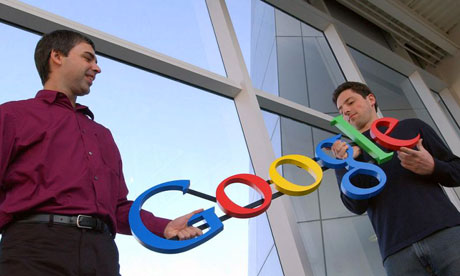
\includegraphics[width=3.5in]{larrysergei.jpg}
\end{center}
\end{frame}


\end{document}

